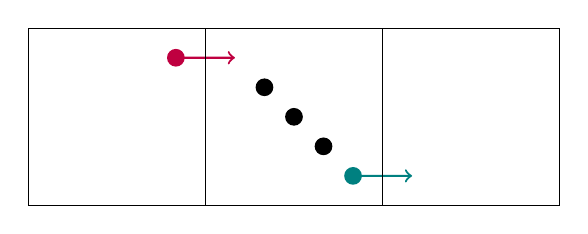
\begin{tikzpicture}[scale=0.75]
    \coordinate (a1) at (5.5,0.5);
    \coordinate (a2) at (5,1);
    \coordinate (a3) at (4.5,1.5);
    \coordinate (a4) at (4,2);
    \coordinate (a5) at (2.5,2.5);
    \draw[purple,->,thick] (a5) -- (3.5,2.5);
    \draw[teal,->,thick] (a1) -- (6.5,0.5);
    \draw (0,0) rectangle (3,3);
    \draw (3,0) rectangle (6,3);
    \draw (6,0) rectangle (9,3);
    \fill[teal] (a1) circle (0.15);
    \fill (a2) circle (0.15);
    \fill (a3) circle (0.15);
    \fill (a4) circle (0.15);
    \fill[purple] (a5) circle (0.15);
\end{tikzpicture}
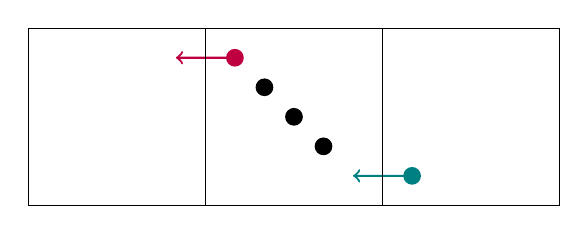
\begin{tikzpicture}[scale=0.75]
    \coordinate (a1) at (6.5,0.5);
    \coordinate (a2) at (5,1);
    \coordinate (a3) at (4.5,1.5);
    \coordinate (a4) at (4,2);
    \coordinate (a5) at (3.5,2.5);
    \draw[purple,->,thick] (a5) -- (2.5,2.5);
    \draw[teal,->,thick] (a1) -- (5.5,0.5);
    \draw (0,0) rectangle (3,3);
    \draw (3,0) rectangle (6,3);
    \draw (6,0) rectangle (9,3);
    \fill[teal] (a1) circle (0.15);
    \fill (a2) circle (0.15);
    \fill (a3) circle (0.15);
    \fill (a4) circle (0.15);
    \fill[purple] (a5) circle (0.15);
\end{tikzpicture}